\section{Measurement Hazards and Negative Results (C3)}

A measurement study is only as credible as its record of what failed, so we keep
a ledger. The flagship entry is a fully diagnosed instrument failure rather than
a missing result, and the diagnosis transfers beyond this dataset.

\textbf{Temporal prediction of recurrence (E5p/E5r): four independent failures.}
Temporal-graph models --- TGN \citep{rossi2020temporal} and the temporal-attention
variant of the same family \citep{xu2020inductive} --- were asked to predict
whether an \textbf{address in the labelled Bitcoin graph} recurs, that is,
whether it is observed in at least two of the 49 ordinal time steps after its
first appearance. They are set against MLP and GraphSAGE \citep{hamilton2017inductive}
baselines, with the instrument gates pre-registered. The target is a recurrence
label on an ordinal axis, not the survival of a social-layer node and not
anchored to an enforcement event, and every model sees only information available
at the address's entry step.

\begin{enumerate}\itemsep1pt
\item \textbf{The predictor lost to its baselines.} On the adjudicated
within-entry-step metric, all three TGN deltas fall below both baselines
(-0.046 to -0.053 against MLP; -0.013 to -0.023 against GraphSAGE).
\item \textbf{The negative-control band self-reported failure, and its report is
separated from its readings.} The band is its own instrument: 400 draws, nominal
window [0.005, 0.055]. Its verbatim verdict is INSTRUMENT FAILED, on exactly
three cells (F1 G1 P1 global D=3 at rate 0.0700, F1 G1 P1 global D=5 at 0.0700,
and F1 G1 P2 within-bin D=5 at 0.0650). Under the two-list rule that report is
the gate's output and we give it in full. No quantity is read from \emph{this}
band, and in particular we publish no ``leakage'' estimate anywhere, because the
excess of the shuffled control over chance conflates feature-side separability
with label leakage and is not decomposable.
\item \textbf{The ablation gate failed, and the family attribution stands on a
different instrument.} The pre-registered ablation gate did not pass, and a
CPU--GPU replicate exceeded tolerance (max $|d|$ = 0.0068 \textgreater{} 1e-3),
so the ablation \emph{estimates} are never tabulated alongside the CPU-series
numbers. That is a prohibition on quantities, not on diagnosis: the per-family
attribution in \S3 is read from the ablation \emph{arm readings}, which carry
their own decision rule, not from the failed estimate.
\item \textbf{The apparent positive result is not licensable.} The increment of
the true model over the shuffled control is +0.05, two point estimates with no
null distribution, and we claim no significance for it.
\end{enumerate}

\textbf{The trap, measured rather than described.} The feature matrix of the
pre-registered plan contains a column that \emph{is} the $\Delta = 1$ label
(\texttt{num\_timesteps\_appeared\_in} $\geq$ 2). A baseline consuming that
matrix reaches test AUC \textbf{1.0}, and the artifact declares the same baseline
inadmissible in the same breath, for exactly that reason. We agree with the
declaration and keep the number because it measures something else --- how
completely a structurally derived label can be re-derived from its own feature
table. It is a measurement of the hazard, not a performance figure.

\textbf{How far the repair goes.} Read on the within-entry-step metric the arms
are judged on, the three de-leakage configurations are not what a summary of
them suggests. Configuration L1 keeps nine of the as-built arm's ten features
(all but the calendar column) and reads \textbf{0.7155632}, \emph{above} the
as-built baseline of \textbf{0.7136417}, so dropping the calendar channel alone
repairs nothing. Configuration L2 keeps three features and reads
\textbf{0.6560979}, a real reduction that still does not reach chance.
Configuration L3 reads exactly \textbf{0.5000} and the artifact marks it at
chance --- but L3 retains only the stratifying variable itself, and a single
feature constant within every bin yields an AUC of exactly one half by
construction. L3 is therefore a vacuous control in the sense \S3 defines, and its
0.5 is not evidence of repair. \textbf{The strongest non-vacuous configuration moves
the control from 0.7136 to 0.6561 and stops there.} (Fig.~\ref{fig4}) The values 0.633 / 0.652 /
0.681 that the same artifact reports are its \emph{pooled} per-horizon figures,
which the artifact itself notes are not comparable to 0.5.

One limitation is declared inside the artifact and repeated here: the
de-leakage removes node and
tabular feature columns, but \textbf{graph message passing still runs over the
full snapshot graph}.

\textbf{A floor worth recording.} An untrained model of the same architecture
already separates at up to \textbf{0.6378} (GraphSAGE, $\Delta = 1$), and across
the three configurations the untrained GraphSAGE readings span
\textbf{0.3672--0.6378}, so any AUC inside that band is architecture rather than
learning. No reported reading is treated as a performance figure until it clears
that floor, which is the same discipline \S3 applies to the metric layer and the
reason the ledger does not stop at a bare failure count.

\textbf{Why this is in the paper.} Within the scope of this data structure and
this label-construction process, an evaluation that shuffles labels without first
demonstrating that the shuffle breaks the feature--label association \emph{inside
each stratification bin} can report an inflated AUC with a clean conscience and a
broken null model. Whether that transfers to other censored, structurally
labelled graphs is a question this paper does not answer. The feature-side
separability trap is an instance of the leakage family that \citet{kapoor2023leakage}
catalogue, and the de-leakage procedure and the vacuous-control test of \S3 are
the paper's reusable countermeasures.

A graph-side de-leakage stage, in which
message passing was restricted to within entry-step strata, was voided by its own
pre-registered replication gate: the mask-off control cells failed bitwise
agreement with the prior generation, and by the registered rule all readings of
that round are withdrawn. A directed attribution run reproduced the non-temporal
models bitwise and isolated the discrepancy to the temporal model's
environment-level nondeterminism, and an independent cross-device comparison
reproduced that attribution under fp64 deterministic mode, where the
non-temporal arms agree bitwise across CPU and GPU while the temporal arm does
not. Cross-environment replication of temporal-graph pipelines is itself a hazard
the protocol is designed to intercept, and this entry records it doing so.

\textbf{Three further dead ends, briefly.} Unsupervised changepoint detection on
temporal embeddings of the market graphs (E14) missed every reference event,
reading a firing rate of \textbf{0/25 = 0.000} and clearing its threshold by
missing rather than by detecting, while a volume-only control does fire (rate
0.040), so the detector is not inert. The originally specified events lie outside
the data's time range, and the substitutions actually used are disclosed in
Supplementary Note S3. Two-event consistency (E2) is infeasible
by pre-registered criterion, because no acquired dataset brackets Operation
Onymous (2014-11) or Bayonet (2017-07), which is why \S\ref{sec:e1v3} measures
the November 2019 shutdowns instead. Role annotation (E10) never reached data
acquisition and no number here depends on it, and external validation against
monthly breach-posture reports (EV-legacy) was rejected as a validation target
for window drift.

\begin{figure}[htbp]
\centering
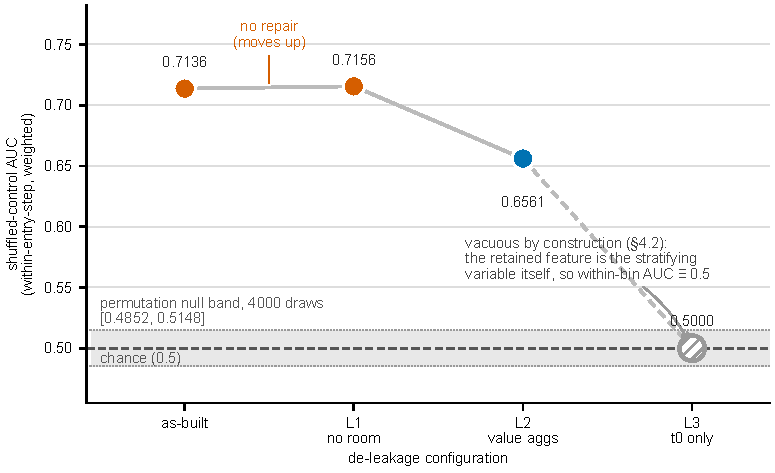
\includegraphics[width=0.50\textwidth]{figures/06_shuffled_trajectory.pdf}
\caption{The shuffled-control trajectory, trap versus post-de-leakage, on the
within-entry-step weighted AUC. The as-built configuration reads 0.7136;
dropping the calendar column alone reads 0.7156, \emph{above} it, so the path
moves the wrong way before it moves right. The strongest non-vacuous
configuration reaches 0.6561 and stops. The final point reads exactly 0.5000 and
is drawn hollow and hatched because it is fixed by construction, not
achieved.\label{fig4}}
\end{figure}
